\documentclass[../main.tex]{subfiles}


\begin{document}
	\section{Práce se senzory}
	
	\subsection{Enkóder}\label{cha:encoder}
	Enkóder je senzor nezbytný k přesnému pohybu robota, jelikož měří otáčky jeho kol. Díky tomu jde (s dobrou přesností) určit, kde se robot nachází, a přizpůsobit tomu i naše programy.

	Jeden z nejčastějších typů enkóderů je optický enkóder. Funguje na principu světelného senzoru, na který svítí světlo (většinou laser). Otáčením kolečka se senzor postupně zakrývá/odkrývá a touto změnou je tedy možné určit, že se kolečko otočilo.

	\begin{figure}
		\centering%
		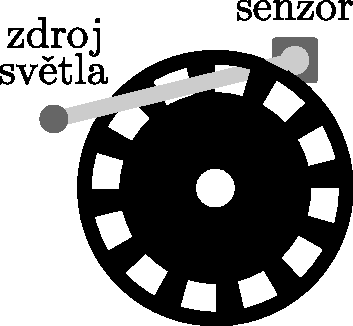
\includegraphics[width=0.25\linewidth]{Images/03/encoder-through.pdf}
		\hspace{.15\textwidth}%
		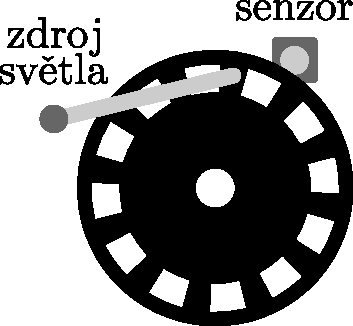
\includegraphics[width=0.25\linewidth]{Images/03/encoder-blocked.pdf}
		\caption{Polohy optického enkóderu; nalevo světlo propouští, napravo blokuje.}
	\end{figure}

	Všechny motory, se kterými náš robot pracují, v sobě už enkóder zabudovaný mají. Využívá ho např. blok \blockMotorDistanceImage (a řada dalších) který na jeho základě měří otáčky kola.

	\begin{question}
		Kolečko nahoře odkrývá a zakrývá senzor, z čehož počítáme uraženou vzdálenost. Dokážeme této informace také určit, jakým směrem se kolečko točí? Pokud ne, kolik koleček na to budeme potřebovat?
	\end{question}

	\begin{solution}
		Nedokážeme, protože střídavým zakrýváním/odkrýváním senzoru můžeme pouze sledovat, že se kolečko otáčí. Ke správnému určení směru je potřeba další kolečko, zdroj světla a senzor, které jsou od původního kolečka o kousek pootočené.

		Nyní už dokážeme pozorovat, zda se nejprve zakryl první senzor a až poté druhý, nebo nejdříve druhý a až poté první, což nám přesně určí směr (a samozřejmě vzdálenost) otáčení.
	\end{solution}

	\subsection{Senzor nárazu}
	Senzor nárazu (anglicky \textit{Bumper Switch}) je další ze senzorů, které budeme k pohybu robota využívat. Hodí se, když budeme chtít rozpoznávat, zda robot náhodou do něčeho nenarazil a např. by se tedy měl otočit a jet jinam. Funguje na velice přímočarém principu -- pokud není stlačen, tak obvod uvnitř není propojený; jakmile stlačen je, tak se obvod propojí.

	\begin{question}
		Přidělejte na zadní část našeho robota dva senzory nárazu.
	\end{question}

	\subsubsection{Nastavení senzoru}
	K připojení senzoru tohoto typu (tři drátky) klikneme na \centerimage{\baselineskip}{Images/ui/gear.png} napravo od písmene, do kterého je senzor na našem robotu zapojený (A-H), vybereme \textbf{Bumper} a stiskneme \textbf{OK}.

	\subsubsection{Programování se senzorem}
	Bloky k programování těchto typů vstupů jsou k nalezení v sekci \textbf{TriPort Input}. Pro senzor nárazu nám bude stačit následující:
	\begin{itemize}
		\blockBumperPressed
	\end{itemize}

	Použijeme ho stejným způsobem, jako jsme používali \blockMotorDoneImage v kapitole \ref{cha:distanceride}. Následující kód naprogramuje robota, aby jel dopředu, dokud se nestiskne jeho senzor nárazu:

	\begin{figure}
		\centering
		\begin{minipage}{0.5\textwidth}
			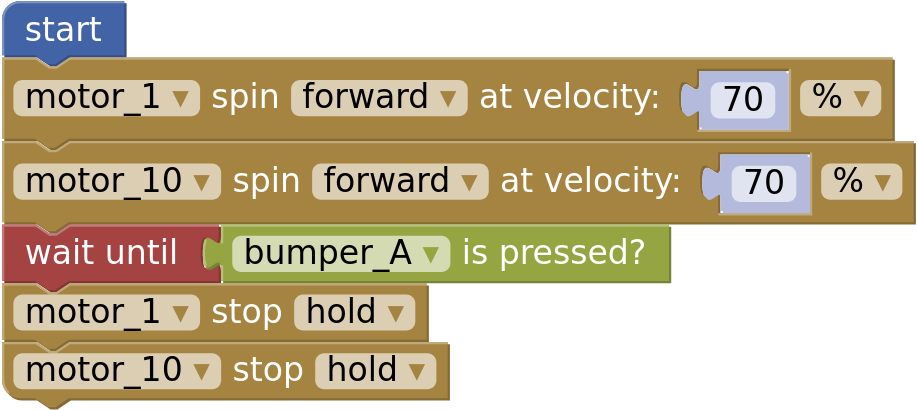
\includegraphics[width=\linewidth]{Images/02/sol7.png}
		\end{minipage}
	\end{figure}

	\begin{question}
		Naprogramujte robota, aby opakovaně prováděl následující:
		\begin{enumerate}
			\item jel dozadu, dokud do něčeho nenarazí (detekujte přes blok ukázaný výše)
			\item po nárazu jel kousek dopředu
			\item otočil se o 90\degree
		\end{enumerate}
	\end{question}
\end{document}
